%-----------------------------------------------------------------------
%
\section{\emph{Intermediate} Tuning for Balanced Servo/Regulation Operation}
\label{methodology}
%
%-----------------------------------------------------------------------

The tuning approaches presented in subsection \ref{tuning-modes}
can be considered extremal situations. The controller settings are
obtained by considering exclusively one mode of operation. This
may generate, as it has been shown in the previous section, quite
poor performance if the non-considered situation happens. This
fact suggests to analyze if, by loosing some degree of optimality
with respect to the tuning mode, the Performance Degradation can
be reduced when the operation is different to the selected one for
tuning.

Based on this observation we suggest to look for an
\emph{intermediate} controller. In order to define this
exploration, we need to define the search-space and the overall
Performance Degradation index to be minimized. Obviously the
solution will depend on how this factors are defined.

The search of the controller settings that provide a
\emph{trade-off} performance for both operating modes could be
stated in terms of a completely new optimization procedure.
However, we would like to take advantage of the autotuning
formulae (like (\ref{set_point_tuning_formulae}) and
(\ref{load_disturbance_tuning_formulae})), in order to keep the
procedure, as well as the resulting controller expression, in
similar simple terms. Therefore, the resulting controller settings
could be considered as an extension of the optimal ones. On this
basis we define a controller settings family parameterized in
terms of a vector as

\be \overline{\gamma} = \left [\gamma_1,
\gamma_2, \gamma_3 \right] \ee

\noindent where $\gamma_i$ is a variable for each controller
parameter ($K_p$, $T_i$, $T_d$) that allows searching for the
\emph{intermediate} tuning. The values for this factor are
restricted to $\gamma_i \in [0,1]\quad i=1,2,3$. Also, the
set-point tuning will correspond to a contour constraint for each
$\gamma_i=0$, whereas the load-disturbance tuning corresponds to
$\gamma_i=1$. Fig. \ref{gamma} shows graphically the procedure and
the application for the 1-DoF PID controller tuning.

\begin{figure}[h!]
    \begin{center}
        %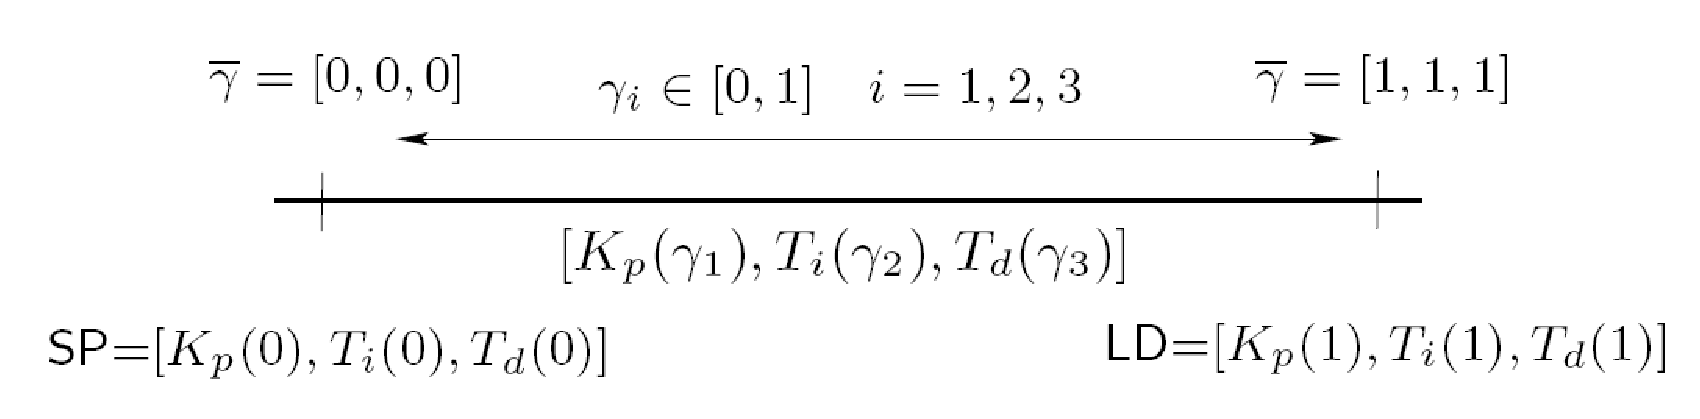
\includegraphics[scale=0.4]{gammaS.eps}
        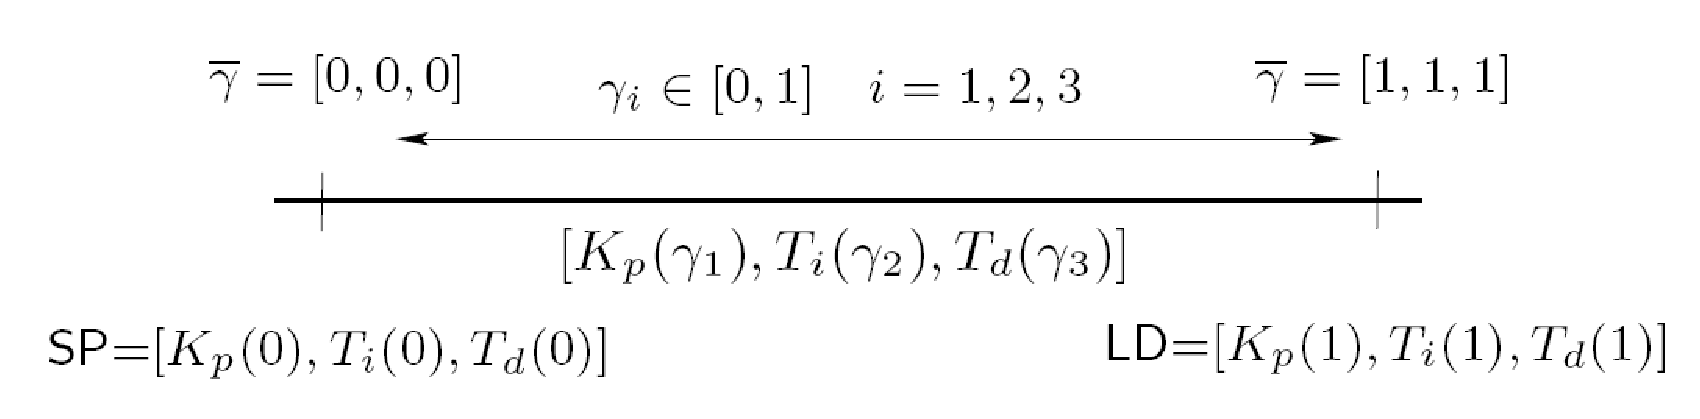
\includegraphics[width=0.8\linewidth]{gammaS.eps}
        \caption{$\overline{\gamma}-tuning$ procedure for the search of the \emph{intermediate} controller.}\label{gamma}
   \end{center}
\end{figure}

The controller settings family $[K_p(\gamma_1), T_i(\gamma_2),
T_d(\gamma_3)]$ will be generated by a linear evolution for the
parameters from the set-point tuning to the load-disturbance one
and the other way around. Therefore,
\bea
K_p(\gamma_1) & = & \gamma_1 K_p^{ld}+ (1-\gamma_1)K_p^{sp} \nonumber \\
T_i(\gamma_2) & = & \gamma_2 T_i^{ld}+ (1-\gamma_2)T_i^{sp} \label{gammaS_tuning_formulae}\\
T_d(\gamma_3) & = & \gamma_3 T_d^{ld}+ (1-\gamma_3)T_d^{sp}
\nonumber \eea

\noindent where $\gamma_i \in [0,1]\quad i=1,2,3$ and $[K_p^{sp},
T_i^{sp}, T_d^{sp}]$ and $[K_p^{ld}, T_i^{ld}, T_d^{ld}]$ stand
for the set-point and load-disturbance settings for $[K_p, T_i,
T_d]$ respectively.

Now, in order to define a global Performance Degradation
($\mathit{PD}$) index, the previously defined terms
(\ref{PD_load_disturbance}) and (\ref{PD_set_point}) need to be
extended. Note that the Performance Degradation was associated to
the \emph{tuning mode}, therefore tested against the opposite
\emph{operating mode}. Now, for every combination of
$\overline{\gamma}$ the Performance Degradation needs to be
measured with respect to both operating modes (because the
corresponding $\overline{\gamma}-tuning$ does not necessarily
corresponds to an operating mode). Hence,

\begin{itemize}
\item $PD_{sp}(\overline{\gamma})$ will represent the Performance
Degradation of the $\overline{\gamma}-tuning$ on servo operating
mode.

\be PD_{sp}(\overline{\gamma}) = \left |
\frac{J_{sp}(\overline{\gamma}) - J_{sp}(sp)}{J_{sp}(sp)} \right |
\label{PD_gamma_servo} \ee

\item $PD_{ld}(\overline{\gamma})$ will represent the Performance
Degradation of the $\overline{\gamma}-tuning$ on regulation
operating mode.

\be PD_{ld}(\overline{\gamma}) = \left |
\frac{J_{ld}(\overline{\gamma}) - J_{ld}(ld)}{J_{ld}(ld)} \right |
\label{PD_gamma_disturbance} \ee
\end{itemize}

From these Performance Degradation definitions, the overall
Performance Degradation is introduced and interpreted as a
function of $\overline{\gamma}$. There may be different ways to
define the $PD(\overline{\gamma})$ function, depending on the
importance associated to every operating mode (e.g. applying
weighting factors to each component). However, every definition
must satisfy the following contour constraints

\begin{displaymath}
PD(\overline{\gamma}) = \left \{ \begin{array}{ll} PD_{ld}(sp) &
\textrm{for  $\overline{\gamma}=\left[0,
0, 0 \right]$}\\
PD_{sp}(ld) & \textrm{for  $\overline{\gamma}=\left[1, 1, 1
\right]$}
\end{array} \right.
\end{displaymath}

The most simple definition would be

\be PD(\overline{\gamma}) =
PD_{ld}(\overline{\gamma}) + PD_{sp}(\overline{\gamma})
\label{global_pd} \ee

This expression represents a compromise, or a balance, between
both losses of performance.

As it has been mentioned before, the greatest loss of performance
occurs when the load-disturbance tuning operates as a servo mode.
Therefore, $PD_{sp}(\overline{\gamma})$ will be the largest
component of the global expression of $PD(\overline{\gamma})$ and
in the oppositive side $PD_{ld}(\overline{\gamma})$ the smallest
one. This causes that the percentage reduction of $\mathit{PD}$
that can be obtained from the $PD_{ld}$ side is lower than the one
for the $PD_{sp}$ part. A balanced reduction of
$PD(\overline{\gamma})$ from both Performance Degradations is
possible by introducing weighting factors associated to each
operating mode \cite{arrietaCSC2007}. This idea can be applied
rewriting (\ref{global_pd}) as

\be WPD(\overline{\gamma};\alpha) = \alpha
PD_{ld}(\overline{\gamma}) + (1-\alpha) PD_{sp}(\overline{\gamma})
\label{alpha_pd} \ee

\noindent that we call Weighted Performance Degradation
($\mathit{WPD}$) index, where $\alpha \in [0,1]$ is the weight
factor and indicates which of the two possible operation modes is
preferred or more important.

One way to express the importance between both operation modes,
could be the total time that the system operates in each one of
them. For example, a system that operates the 75\% of the time as
a regulator (or viceversa 25\% as a servo), $\alpha=0.75$.
However, the $\alpha$ parameter allows to make a more general
choice for the preference of the system operation (not only taking
into account the time for each operation mode).

Note also that (\ref{alpha_pd}) with $\alpha=0.50$, represents an
equivalent expression obtained previously in (\ref{global_pd})
that gives the same significance for both operation modes.

The \emph{intermediate} tuning will be determined by proper
selection of $\overline{\gamma} = \left [\gamma_1, \gamma_2,
\gamma_3 \right]$. This choice will correspond to the solution of
the following optimization problem,

\be \overline{\gamma}_{op} := \left [\gamma_{1op}, \gamma_{2op},
\gamma_{3op} \right ] = arg \left
[\min_{\overline{\gamma}}WPD(\overline{\gamma};\alpha) \right ]
\label{gamma_optimization}\ee

It is obvious that $\alpha=0$ means
\be WPD(\overline{\gamma};0) =
PD_{sp}(\overline{\gamma}) \label{alpha_pd0} \ee

\noindent and of course the $\overline{\gamma}_{op}$ that
minimizes the Performance Degradation for servo operation mode
(\ref{alpha_pd0}), is the one that corresponds to the set-point
tuning ($\overline{\gamma}=[0,0,0]$). On the other side,
$\alpha=1$ is equivalent to

\be WPD(\overline{\gamma};1) = PD_{ld}(\overline{\gamma})
\label{alpha_pd1} \ee

\noindent and the tuning that minimizes the Performance
Degradation for regulation operation (\ref{alpha_pd1}) is the
load-disturbance tuning that equals to
$\overline{\gamma}=[1,1,1]$.

The optimal values (\ref{gamma_optimization}) jointly with
(\ref{gammaS_tuning_formulae}), give a tuning formula that
provides a worse performance than the optimal settings operating
in the same way but also a lower degradation in the performance
when the \emph{operating mode} is different from the \emph{tuning
mode}.
